\documentclass[tikz,border=12pt]{standalone}
\usepackage{helvet}
\usepackage{amsmath,amssymb}
\renewcommand{\familydefault}{\sfdefault}
\usepackage{tikz}
\usepackage{tikz-3dplot}
\usetikzlibrary{calc, positioning, shapes, arrows.meta}

\definecolor{emeraldpine}{HTML}{1A4D3E}
\definecolor{harvardcrimson}{HTML}{A51C30}
\definecolor{ethdarkblue}{HTML}{1F407A}
\definecolor{ethpetrol}{HTML}{007A87}
\definecolor{ethbronze}{HTML}{B87333}
\definecolor{ink}{HTML}{1A202C}
\definecolor{cardbg}{HTML}{F8FAFC}
\definecolor{shadecolor}{HTML}{F4F6F9}
\definecolor{paleink}{HTML}{94A3B8}

\begin{document}
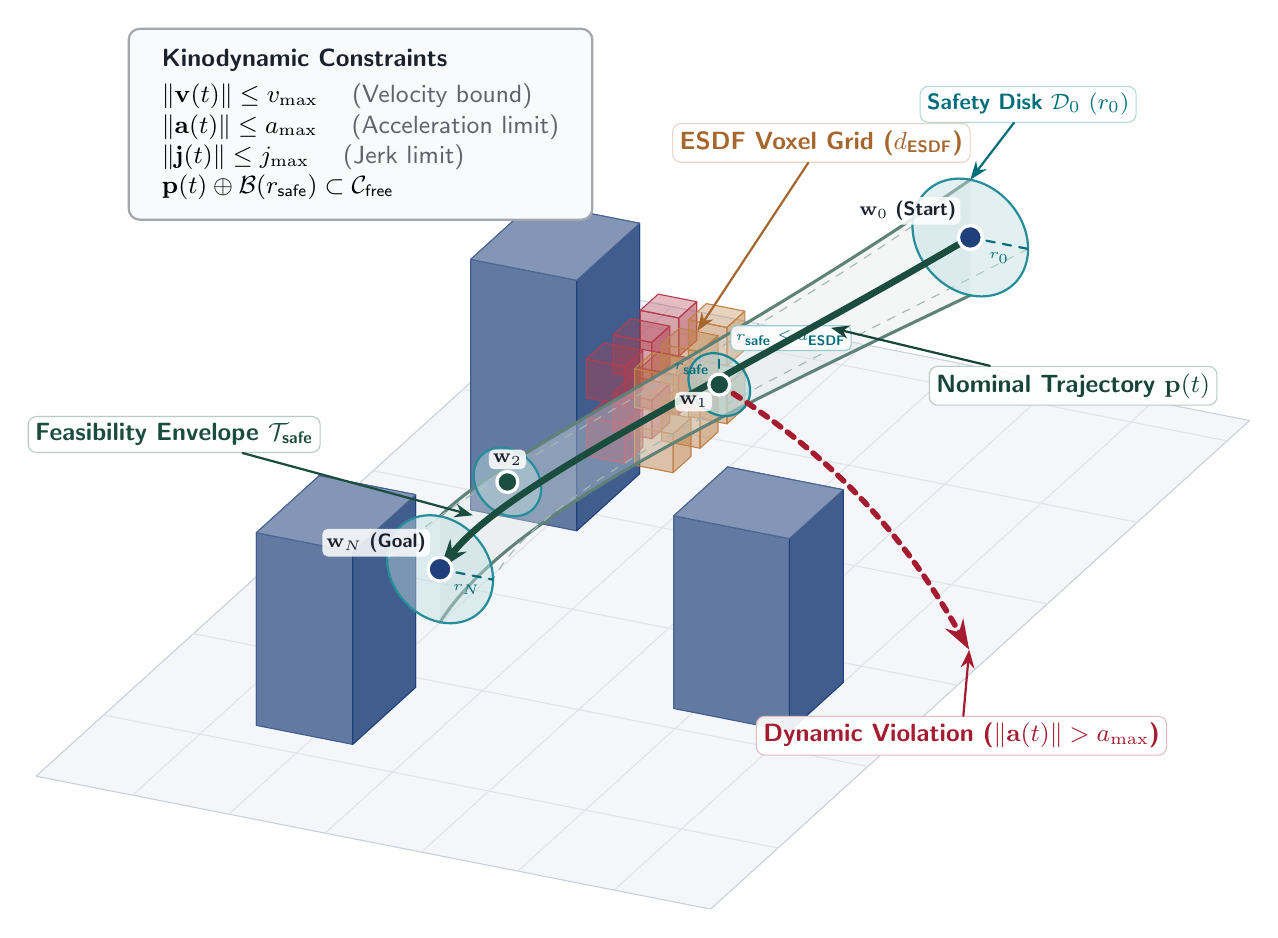
\begin{tikzpicture}[font=\sffamily, >=Stealth]

\tdplotsetmaincoords{65}{115}
\begin{scope}[tdplot_main_coords, scale=1.35, line join=round, line cap=round]

% Ground plane
\fill[shadecolor] (-1.5,-3.0,0) -- (10.5,-3.0,0) -- (10.5,4.0,0) -- (-1.5,4.0,0) -- cycle;
\draw[paleink!50, thin] (-1.5,-3.0,0) -- (10.5,-3.0,0) -- (10.5,4.0,0) -- (-1.5,4.0,0) -- cycle;

% Grid lines
\foreach \gx in {-1, 1, 3, 5, 7, 9} {
    \draw[paleink!30, thin] (\gx, -3.0, 0) -- (\gx, 4.0, 0);
}
\foreach \gy in {-2, -1, 0, 1, 2, 3} {
    \draw[paleink!30, thin] (-1.5, \gy, 0) -- (10.5, \gy, 0);
}

% Macro for drawing 3D box (x, y, z, dx, dy, dz)
\newcommand{\drawblock}[6]{
  \filldraw[fill=ethdarkblue!90, draw=ethdarkblue!95, thin]
    (#1,#2,#3) -- (#1+#4,#2,#3) -- (#1+#4,#2,#3+#6) -- (#1,#2,#3+#6) -- cycle;
  \filldraw[fill=ethdarkblue!80, draw=ethdarkblue!90, thin]
    (#1,#2,#3) -- (#1,#2+#5,#3) -- (#1,#2+#5,#3+#6) -- (#1,#2,#3+#6) -- cycle;
  \filldraw[fill=ethdarkblue!70, draw=ethdarkblue!85, thin]
    (#1+#4,#2,#3) -- (#1+#4,#2+#5,#3) -- (#1+#4,#2+#5,#3+#6) -- (#1+#4,#2,#3+#6) -- cycle;
  \filldraw[fill=ethdarkblue!85, draw=ethdarkblue, thin]
    (#1,#2+#5,#3) -- (#1+#4,#2+#5,#3) -- (#1+#4,#2+#5,#3+#6) -- (#1,#2+#5,#3+#6) -- cycle;
  \filldraw[fill=ethdarkblue!55, draw=ethdarkblue!80, thin]
    (#1,#2,#3+#6) -- (#1+#4,#2,#3+#6) -- (#1+#4,#2+#5,#3+#6) -- (#1,#2+#5,#3+#6) -- cycle;
}

% Macro for drawing voxel cube (x, y, z, size, color)
\newcommand{\drawvoxel}[5]{
  \filldraw[fill=#5, fill opacity=0.35, draw=#5, thin]
    (#1,#2,#3+#4) -- (#1+#4,#2,#3+#4) -- (#1+#4,#2+#4,#3+#4) -- (#1,#2+#4,#3+#4) -- cycle;
  \filldraw[fill=#5, fill opacity=0.45, draw=#5, thin]
    (#1+#4,#2,#3) -- (#1+#4,#2+#4,#3) -- (#1+#4,#2+#4,#3+#4) -- (#1+#4,#2,#3+#4) -- cycle;
  \filldraw[fill=#5, fill opacity=0.55, draw=#5, thin]
    (#1,#2+#4,#3) -- (#1+#4,#2+#4,#3) -- (#1+#4,#2+#4,#3+#4) -- (#1,#2+#4,#3+#4) -- cycle;
}

% BACKGROUND OBSTACLE 1 (Left/back side: x in [2.0, 3.4], y in [-1.8, -0.7], z in [0, 2.6])
\drawblock{2.0}{-1.8}{0}{1.4}{1.1}{2.6}

% ESDF Voxels around Obstacle 1 (gradient from obstacle towards path)
% Red: close to obstacle surface (danger / small distance)
\foreach \vx in {1.8, 2.4, 3.0} {
  \drawvoxel{\vx}{-0.6}{0.8}{0.4}{harvardcrimson!85}
  \drawvoxel{\vx}{-0.6}{1.4}{0.4}{harvardcrimson!85}
}
% Amber: safety margin (medium distance)
\foreach \vx in {1.8, 2.4, 3.0} {
  \drawvoxel{\vx}{-0.1}{0.8}{0.4}{ethbronze!90}
  \drawvoxel{\vx}{-0.1}{1.4}{0.4}{ethbronze!90}
}

% BACKGROUND OBSTACLE 3 (Far left/exit side: x in [7.2, 8.6], y in [-1.6, -0.6], z in [0, 2.0])
\drawblock{7.2}{-1.6}{0}{1.4}{1.0}{2.0}

% Waypoint Coordinates
\coordinate (P0) at (0.0, 1.8, 2.1);
\coordinate (P1) at (2.8, 0.5, 1.5);
\coordinate (P2) at (5.8, -0.3, 1.6);
\coordinate (P3) at (8.8, 0.4, 2.1);

\def\rZero{0.60}
\def\rOne{0.32}
\def\rTwo{0.35}
\def\rThree{0.55}

% Tube sheath fill (translucent feasibility envelope)
\fill[emeraldpine!15, fill opacity=0.35]
  (0.0, 1.8, 2.1+\rZero) .. controls (2.8, 0.5, 1.5+\rOne) and (5.8, -0.3, 1.6+\rTwo) .. (8.8, 0.4, 2.1+\rThree)
  -- (8.8, 0.4, 2.1-\rThree) .. controls (5.8, -0.3, 1.6-\rTwo) and (2.8, 0.5, 1.5-\rOne) .. (0.0, 1.8, 2.1-\rZero)
  -- cycle;

% Boundary rails
\draw[emeraldpine!70, line width=1.1pt]
  (0.0, 1.8, 2.1+\rZero) .. controls (2.8, 0.5, 1.5+\rOne) and (5.8, -0.3, 1.6+\rTwo) .. (8.8, 0.4, 2.1+\rThree);
\draw[emeraldpine!70, line width=1.1pt]
  (0.0, 1.8, 2.1-\rZero) .. controls (2.8, 0.5, 1.5-\rOne) and (5.8, -0.3, 1.6-\rTwo) .. (8.8, 0.4, 2.1-\rThree);

\draw[emeraldpine!40, thin, dashed]
  (0.0, 1.8+\rZero, 2.1) .. controls (2.8, 0.5+\rOne, 1.5) and (5.8, -0.3+\rTwo, 1.6) .. (8.8, 0.4+\rThree, 2.1);
\draw[emeraldpine!40, thin, dashed]
  (0.0, 1.8-\rZero, 2.1) .. controls (2.8, 0.5-\rOne, 1.5) and (5.8, -0.3-\rTwo, 1.6) .. (8.8, 0.4-\rThree, 2.1);

% Safety Disks at cross-sections
% Disk 0 (Start)
\begin{scope}[canvas is yz plane at x=0.0]
  \filldraw[fill=ethpetrol!25, draw=ethpetrol!85, thick, fill opacity=0.45] (1.8, 2.1) circle (\rZero);
  \draw[dashed, ethpetrol!90!black, thick] (1.8, 2.1) -- +(\rZero, 0);
  \node[font=\tiny\bfseries, text=ethpetrol!90!black, below] at (1.8+\rZero/2, 2.1) {$r_0$};
\end{scope}

% Disk 1 (Constriction)
\begin{scope}[canvas is yz plane at x=2.8]
  \filldraw[fill=ethpetrol!30, draw=ethpetrol!90, thick, fill opacity=0.55] (0.5, 1.5) circle (\rOne);
  \draw[dashed, ethpetrol!90!black, thick] (0.5, 1.5) -- +(0, \rOne);
  \node[font=\tiny\bfseries, text=ethpetrol!90!black, left] at (0.5, 1.5+\rOne/2) {$r_{\text{safe}}$};
  \node[font=\tiny\bfseries, text=ethpetrol!90!black, fill=white, fill opacity=0.9, text opacity=1, inner sep=1.8pt, rounded corners=2pt, draw=ethpetrol!40, above right=1pt and 4pt] at (0.5, 1.5+\rOne) {$r_{\text{safe}} \le d_{\text{ESDF}}$};
\end{scope}

% Disk 2 (Middle curve)
\begin{scope}[canvas is yz plane at x=5.8]
  \filldraw[fill=ethpetrol!25, draw=ethpetrol!85, thick, fill opacity=0.45] (-0.3, 1.6) circle (\rTwo);
\end{scope}

% Disk 3 (Goal)
\begin{scope}[canvas is yz plane at x=8.8]
  \filldraw[fill=ethpetrol!25, draw=ethpetrol!85, thick, fill opacity=0.45] (0.4, 2.1) circle (\rThree);
  \draw[dashed, ethpetrol!90!black, thick] (0.4, 2.1) -- +(\rThree, 0);
  \node[font=\tiny\bfseries, text=ethpetrol!90!black, below] at (0.4+\rThree/2, 2.1) {$r_N$};
\end{scope}

% Nominal Trajectory
\draw[emeraldpine, line width=2.4pt, -{Stealth[length=3.8mm, width=2.6mm]}]
  (P0) .. controls (2.8, 0.5, 1.5) and (5.8, -0.3, 1.6) .. (P3);

% FOREGROUND OBSTACLE 2 (Right/front side: x in [5.4, 6.6], y in [1.8, 3.0], z in [0, 2.0])
\drawblock{5.4}{1.8}{0}{1.2}{1.2}{2.0}

% Dynamic Violation Curve (diverges from P1, sweeping out in foreground towards bottom right)
\draw[harvardcrimson, line width=2.0pt, dashed, -{Stealth[length=3.8mm, width=2.6mm]}]
  (P1) .. controls (3.8, 2.4, 1.4) and (4.8, 3.5, 1.1) .. (5.6, 4.4, 0.7);

% Waypoint Node Markers
\filldraw[fill=ethdarkblue, draw=white, line width=1.2pt] (P0) circle (3.2pt)
  node[above left, font=\scriptsize\bfseries, text=ink, fill=white, fill opacity=0.85, text opacity=1, inner sep=1.5pt, rounded corners=2pt, xshift=-3pt, yshift=4pt] {$\mathbf{w}_0$ (Start)};

\filldraw[fill=emeraldpine, draw=white, line width=1.2pt] (P1) circle (2.8pt)
  node[below left, font=\scriptsize\bfseries, text=ink, fill=white, fill opacity=0.85, text opacity=1, inner sep=1.5pt, rounded corners=2pt, xshift=-2pt, yshift=-2pt] {$\mathbf{w}_1$};

\filldraw[fill=emeraldpine, draw=white, line width=1.2pt] (P2) circle (2.8pt)
  node[above, font=\scriptsize\bfseries, text=ink, fill=white, fill opacity=0.85, text opacity=1, inner sep=1.5pt, rounded corners=2pt, yshift=4pt] {$\mathbf{w}_2$};

\filldraw[fill=ethdarkblue, draw=white, line width=1.2pt] (P3) circle (3.2pt)
  node[above left, font=\scriptsize\bfseries, text=ink, fill=white, fill opacity=0.85, text opacity=1, inner sep=1.5pt, rounded corners=2pt, xshift=-3pt, yshift=4pt] {$\mathbf{w}_N$ (Goal)};

% 3D Callout Nodes and Leader Lines
% 1. Nominal Trajectory: placed in foreground-right open space, pointing directly to trajectory
\node[emeraldpine!90!black, font=\small\bfseries, fill=white, fill opacity=0.9, text opacity=1, inner sep=2.5pt, rounded corners=3pt, draw=emeraldpine!30]
  (nom_lbl) at (2.0, 3.8, 1.8) {Nominal Trajectory $\mathbf{p}(t)$};
\draw[emeraldpine!90!black, thick, ->] (nom_lbl) -- (1.6, 1.1, 1.7);

% 2. Safety Disk callout (Disk 0)
\node[ethpetrol!90!black, font=\footnotesize\bfseries, fill=white, fill opacity=0.9, text opacity=1, inner sep=2.5pt, rounded corners=3pt, draw=ethpetrol!30]
  (disk_lbl) at (0.0, 2.4, 3.6) {Safety Disk $\mathcal{D}_0 \ (r_0)$};
\draw[ethpetrol!90!black, thick, ->] (disk_lbl) -- (0.0, 1.8, 2.1+\rZero);

% 3. ESDF Voxel Grid callout (positioned clearly in open sky to the right of constraints card)
\node[ethbronze!90!black, font=\small\bfseries, fill=white, fill opacity=0.9, text opacity=1, inner sep=2.5pt, rounded corners=3pt, draw=ethbronze!30]
  (esdf_lbl) at (1.6, 1.0, 3.6) {ESDF Voxel Grid ($d_{\text{ESDF}}$)};
\draw[ethbronze!90!black, thick, ->] (esdf_lbl) -- (2.0, -0.1, 1.6);

% 4. Feasibility Envelope callout
\node[emeraldpine, font=\small\bfseries, fill=white, fill opacity=0.9, text opacity=1, inner sep=2.5pt, rounded corners=3pt, draw=emeraldpine!30]
  (tube_lbl) at (8.5, -2.5, 2.8) {Feasibility Envelope $\mathcal{T}_{\text{safe}}$};
\draw[emeraldpine, thick, ->] (tube_lbl) -- (7.0, -0.1, 1.8);

% 5. Dynamic Violation callout
\node[harvardcrimson, font=\small\bfseries, fill=white, fill opacity=0.9, text opacity=1, inner sep=2.5pt, rounded corners=3pt, draw=harvardcrimson!30]
  (violation_lbl) at (6.2, 4.6, 0.1) {Dynamic Violation ($\|\mathbf{a}(t)\| > a_{\max}$)};
\draw[harvardcrimson, thick, ->] (violation_lbl) -- (5.6, 4.4, 0.7);

\end{scope}

% Kinodynamic Constraints Card in upper-left sky
\node[anchor=north west, font=\small\sffamily, fill=cardbg, draw=ink!40, line width=0.8pt, rounded corners=4pt, inner sep=6pt] 
  at (-8.5, 4.8) {
  \begin{tabular}{l}
    \textbf{\textcolor{ink}{Kinodynamic Constraints}} \\[2pt]
    $\|\mathbf{v}(t)\| \le v_{\max}$ \quad \textcolor{ink!70}{(Velocity bound)} \\
    $\|\mathbf{a}(t)\| \le a_{\max}$ \quad \textcolor{ink!70}{(Acceleration limit)} \\
    $\|\mathbf{j}(t)\| \le j_{\max}$ \quad \textcolor{ink!70}{(Jerk limit)} \\
    $\mathbf{p}(t) \oplus \mathcal{B}(r_{\text{safe}}) \subset \mathcal{C}_{\text{free}}$
  \end{tabular}
};

\end{tikzpicture}
\end{document}
